% Copyright (c) 2020 Matematyka dla Ciekawych Świata (http://ciekawi.icm.edu.pl/)
% Copyright (c) 2020 Robert Ryszard Paciorek <rrp@opcode.eu.org>
% Copyright (c) 2020 Krzysztof Lasocki <krz.lasocki@gmail.com>
% 
% MIT License
% 
% Permission is hereby granted, free of charge, to any person obtaining a copy
% of this software and associated documentation files (the "Software"), to deal
% in the Software without restriction, including without limitation the rights
% to use, copy, modify, merge, publish, distribute, sublicense, and/or sell
% copies of the Software, and to permit persons to whom the Software is
% furnished to do so, subject to the following conditions:
% 
% The above copyright notice and this permission notice shall be included in all
% copies or substantial portions of the Software.
% 
% THE SOFTWARE IS PROVIDED "AS IS", WITHOUT WARRANTY OF ANY KIND, EXPRESS OR
% IMPLIED, INCLUDING BUT NOT LIMITED TO THE WARRANTIES OF MERCHANTABILITY,
% FITNESS FOR A PARTICULAR PURPOSE AND NONINFRINGEMENT. IN NO EVENT SHALL THE
% AUTHORS OR COPYRIGHT HOLDERS BE LIABLE FOR ANY CLAIM, DAMAGES OR OTHER
% LIABILITY, WHETHER IN AN ACTION OF CONTRACT, TORT OR OTHERWISE, ARISING FROM,
% OUT OF OR IN CONNECTION WITH THE SOFTWARE OR THE USE OR OTHER DEALINGS IN THE
% SOFTWARE.

\documentclass{pdfBooklets}

\usepackage{tikz}
\usetikzlibrary{circuits.ee.IEC}
\title{Warsztat Elektroniczny}
\author{%
	Projekt ,,Matematyka dla Ciekawych Świata'',\\
	Krzysztof Lasocki\\\normalsize\ttfamily <krz.lasocki@gmail.com>
}
\date  {2020-04-27}

\makeatletter\hypersetup{
	pdftitle = {\@title}, pdfauthor = {\@author}
}\makeatother


\newtcolorbox{Ramka}[1][]{
	colback=white,
	colbacktitle=white,
	coltitle=black,
	colframe=white!50!black,
	fontupper=\small,
	enhanced,
	before skip=13pt plus 2pt,
	#1
}
% Symbol DC

\newcommand{\mathdirectcurrent}{\mathrel{\mathpalette\mathdirectcurrentinner\relax}}
\newcommand{\mathdirectcurrentinner}[2]{%
  \settowidth{\dimen0}{$#1=$}%
  \vbox to .85ex {\offinterlineskip
    \hbox to \dimen0{\hss\leaders\hrule\hskip.85\dimen0\hss}
    \vskip.35ex
    \hbox to \dimen0{\hss
      \leaders\hrule\hskip.17\dimen0
      \hskip.17\dimen0
      \leaders\hrule\hskip.17\dimen0
      \hskip.17\dimen0
      \leaders\hrule\hskip.17\dimen0
    \hss}
    \vfill
  }%
}
% symbol diody
\newcommand\esymbol[1]{\tikz[circuit ee IEC] \draw (0,0) -- (.1,0) node [#1,anchor=west,name=s] {} (s.east) -- +(.1,0);}

\newcommand{\textdirectcurrent}{\mathdirectcurrentinner{\textstyle}{}}

\begin{document}

\maketitle

Elektronika to dziedzina nauki zajmująca się praktycznym wykorzystaniem prądu elektrycznego w postaci sygnałów do przetwarzania
informacji. Aby sprawnie eksplorować tę dziedzinę, warto rozpocząć od zapoznania się z podstawowymi pojęciami i narzędziami w
elektronice. Ten skrypt opisuje elementy niezbędne do pracy w małym warsztacie, który umożliwi Ci eksperymenty elektroniczne.
Omówimy obsługę multimetru oraz przetwornicy, a także podstawy lutowania i bezpieczeństwa pracy w domowym warsztacie elektronicznym.

\section{Obsługa multimetru}

Multimetr (zwany też miernikiem) to podstawowy przyrząd pomiarowy każdego elektronika. Zgodnie z nazwą posiada wiele funkcji pomiarowych.
Najczęściej są to woltomierz (do pomiaru napięcia stałego \textbf{V$\mathdirectcurrent$} i zmiennego \textbf{V$\sim$}),
amperomierz (do pomiaru natężenia prądu stałego \textbf{A$\mathdirectcurrent$} i zmiennego \textbf{A$\sim$}, potocznie zwanego prądem)
oraz omomierz (do pomiaru rezystancji, \textbf{$\Omega$}). Często multrimetr posiada także funkcje:
\begin{itemize}
\item \textbf{Test połączeń} (\textit{continuity mode}), oznaczany symbolem fali dźwiękowej (lub nuty), służy do sprawdzania połączeń elektrycznych.
  Miernik wydaje dźwięk jeśli między sondami pomiarowymi (przewodami) jest połączenie.
\item \textbf{Pomiar diod} (\textit{diode check}), oznaczony symbolem diody \esymbol{diode}, służy do sprawdzania diod i innych elementów półprzewodnikowych.
  Wyświetla spadek napięcia na testowanym złączu półprzewodnikowym.
\item \textbf{Test tranzystorów} (pomiar h\textsubscript{FE}), służący do pomiaru wzmocnienia tranzystora. Najczęściej posiada oddzielne gniazdo
  na mierniku.
\item \textbf{Pomiar pojemności}, oznaczany symbolem \esymbol{capacitor} służy do pomiarów pojemności kondensatorów
\item \textbf{Pomiar temperatury}, ocznaczany symbolem \textbf{$^{\circ}$C} najczęściej za pomocą termopary (dołączana do miernika).
\end{itemize}

Multimetr zachowuje się tak jak przyrząd pomiarowy, którego funkcjonalność jest aktualnie wybrana. Oznacza to że należy go podłączać
tak samo, jak odpowiednie przyrządy pomiarowe. 

\subsection{Połączenie miernika}
W zależności od modelu, multimetr może posiadać od dwóch do czterech gniazd na przewody. Są to:
\begin{itemize}
\item Masa, oznaczana \textbf{COM} (od słowa \textit{common}). Tutaj podłącza się czarny przewód
\item Wejście pomiarowe dla woltomierza, ozn. symbolem \textbf{V}. Często także jest to wejście omomierza, oznaczone \textbf{$\Omega$},
  oraz testu diod (ozn. symbolem diody \esymbol{diode})
\item Wejście miliamperomierza, oznaczone symbolem \textbf{mA}. Jeżeli Twój miernik posiada trzy wejścia, to najczęściej jest ono
  tym samym wejściem, co wejście woltomierza.
\item Wejście amperomierza, oznaczone symbolem \textbf{A}. Najczęściej również jest obok niego podany maksymalny dopuszczalny prąd
  oraz czas pomiaru.
\end{itemize}

\begin{Ramka}{}\begin{center}
  {\noindent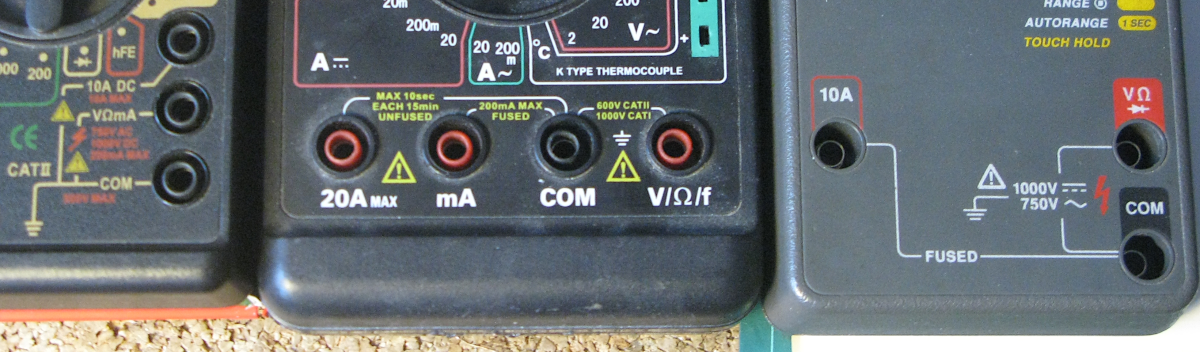
\includegraphics[width=0.99\textwidth,clip=true]{dmm_terminals.png}}\\
  \small
  Wejścia trzech różnych multimetrów. Pomiędzy wejściami zaznaczone są maksymalne wartości napięcia lub natężenia i informacja o zabezpieczeniach  (``FUSED'') bądź ich braku (``UNFUSED'').\\
  Od lewej: typowy model z trzema wejściami, model z czterema wejściami, model z trzema wejściami (bez miliamperomierza)
\end{center}\end{Ramka}

Przy wyborze multimetru należy zwrócić uwagę na jego wejścia. Modele z czterema wejściami są preferowane (zapewnia to izolację funkcji woltomierza
od amperomierza). Przyrząd musi być też opisany jako ``FUSED'', czyli posiadać bezpiecznik na zakresie miliamperomierza (oraz opcjonalnie,
także amperomierza). Pozwoli to uniknąć uszkodzenia multimetru w wypadku przekroczenia dopuszczalnego natężenia prądu.

\subsection{Woltomierz}
Woltomierz to przyrząd służący do pomiaru napięcia elektrycznego między dwoma punktami. Z tego powodu
\textbf{woltomierz podłączamy równolegle} do elementu, który badamy, lub między dwoma punktami w układzie. Opór woltomierza jest możliwie duży (rzeczywiste
woltomierze mają opór około 1-10 M$\Omega$, woltomierz idealny ma opór nieskoczenie wysoki).

\subsection{Amperomierz}
Amperomierz (tudzież miliamperomierz) służy do pomiaru prądu płynącego w gałęzi obwodu. Z tego powodu
\textbf{amperomierz podłączamy szeregowo} z innymi elementami obwodu. Opór amperomierza jest możliwie mały (idealny amperomierz
ma nieskończenie niski opór).
\\

Podłączenie amperomierza równolegle powoduje zwarcie. Nie należy więc odkładać miernika ustawionego na zakres amperów, szczególnie
w przypadku modeli, które używają tego samego gniazda do pomiaru oporności lub napięcia. Skutki pomyłki mogą być fatalne dla
urządzenia - bezpiecznik się spali.

\subsection{Omomierz}
Omomierz jest przyrządem służącym do pomiaru oporności. Jego zasada działania jest dosyć prosta. Składa się on ze źrodła małego napięcia, które pojawia się na końcówkach przewodów pomiarowych. Gdy przyłożymy sondy do elementu mierzonego, omomierz zmierzy jaki prąd płynie przez element testowany i wyświetli jego opór.
\\

Omomierz w praktyce służy tylko do pomiarów oporników. Trzeba pamiętać o tym, że jeżeli mierzymy element umieszczony w układzie,
to jego oporność będzie zawsze niższa od oczekiwanej. Taki opornik jest połączony równolegle z innymi elementami obwodu o
nieznanym oporze, skąd wynika błąd pomiaru.
Zasadniczo nie wykonuje się za jego pomocą pomiarów oporników we włączonych układach.
\\

Przy pomiarach większych oporników (ponad 100k$\Omega$) należy uważać aby nie dotykać palcami końcówek sond, ponieważ opór Twojego ciała
zaniży pomiar. Lepiej jest położyć opornik na stole i przycisnąć jego nóżki za pomocą końcówek sond.


\subsection{Inne funkcje multimetrów}
Oprócz podstawowych funkcji (pomiaru napięcia, natężenia i oporu)\footnotemark, większość nowoczesnych multimetrów posiada także funkcje pomiaru diod oraz tranzystorów.
\\

Funkcja pomiaru diod jest najczęściej oznaczona symbolem diody półprzewodnikowej (\esymbol{diode}) i korzysta z tej samej pary złącz, co woltomierz i omomierz.
Aby zmierzyć spadek napięcia na diodzie należy dotknąć sondą podłączoną do masy (COM) do katody, a sondą dodatnią do anody. Miernik wyświetli
spadek napęcia na złączu diody. Jeżeli miernik wskazuje wynik poza skalą, może to oznaczać, że polaryzacja diody jest odwrotna (sondy są przyłożone na odwrót).
Może też okazać się, że spadek napięcia na jej złączu jest większy niż zakres pomiaru (który najczęściej wynosi do 2V).
\\

\footnotetext{Mierniki, które posiadają tylko te trzy funkcje nazywane są po angielsku VOM (Volt-ohm-milliammeter). Najczęściej są to mierniki
  analogowe.}

Funkcja pomiaru współczynnika wzmocnienia tranzystora bipolarnego jest z reguły oznaczana \textbf{hFE} (od symbolu stosowanego do
oznaczenia tej wartości $\text{h}_{FE}$)\footnote{Czasami oznaczanego też jako $\beta$, beta.}. Pomiar tranzystora za pomocą multimetru polega na umieszczeniu jego nóżek w \textbf{odpowiedni sposób} w gnieździe pomiarowym
w multimetrze. Jego emiter, baza oraz kolektor (oznaczane \textbf{E}, \textbf{B} i \textbf{C} odpowiednio) muszą trafić w
otwory w odpowiedniej połowie gniazda (\textbf{PNP} oraz \textbf{NPN} zależnie od typu tranzystora). Trzeba go obrócić tak, żeby emiter trafił do \textbf{E}, baza do \textbf{B} a kolektor do \textbf{C}. Gniadzo jest tak skontstruowane, że
pasują do niego tranzystory o dowolnej kolejności wyprowadzeń. Kolejność dla Twojego tranzystora jest opisana w jego karcie katalogowej.
Po umieszczeniu tranzystora w gnieździe, na ekranie miernika pojawia się wartość jego współczynnika wzmocnienia $\text{h}_{FE}$.
% \todo{umieścić zdjęcie pokazujące to gniazdo}
\\

Niektóre mierniki posiadają także funkcje pomiaru pojemności elektrycznej kondensatora. W zależności od konstrukcji połączenie testowanego
kondensatora odbywa się poprzez umieszczenie go w specjalnym gnieździe na obudowie miernika albo przez podłączenie sond do wyprowadzeń kondensatora. Należy pamiętać
o tym, że trzeba ustawić zakres w podobny sposób jak przy innych pomiarach. Uwaga - \textbf{nie należy mierzyć pojemności naładowanych
  kondensatorów}. Funkcja pomiaru pojemności przydaje się przy sprawdzaniu kondensatorów ceramicznych lub foliowych o pojemnościach od kilku nF do kilkudziesięciu uF. Na kondensatorach elektrolitycznych lub tantalowych (o większych pojemnościach) wartość
pojemności jest z reguły napisana na obudowie.

\begin{ProTip}{\normalfont{\strong{Uwaga}}}
  Kondensatory elektrolityczne oraz tantalowe są elementami \textbf{spolaryzowanymi}. Podłączając je, należy pamiętać o polaryzacji i podłączać je
  tylko zgodnie z polaryzacją - biegun ujemny do punktu o niższym napięciu, a biegun dodatni do punktu o wyższym napięciu. Na tych kondensatorach jeden
  z biegunów (najczęściej ujemny) jest zaznaczony na obudowie.
  
  \textbf{Uwaga:} Niewłaściwe podłączenie kondensatora może doprowadzić do jego eksplozji.
  Dla własnego bezpieczeństwa nie rób tego – jeżeli jesteś ciekawy jak to wygląda obejrzyj filmik w Internecie.
  Pamiętaj o tym także montując kondensator w swoich konstrukcjach.
\end{ProTip}

Oprócz opisanych wyżej funkcji, niektóre multimetry mogą mieć także funkcje pomiaru temperatury (poprzez \textbf{termoparę}
lub \textbf{termistor} podłączane do
specjalnego złącza na mierniku) oraz pomiar częstotliwości.

\subsection{Dokonywanie pomiarów}

Zależnie od wielkości fizycznej, którą chcemy zmierzyć, czerwony (dodatni) przewód miernika musi być podłączony do odpowiadającego
mu gniazda. Czarny przewód (ujemny, masa) należy zawsze podłączyć do gniazda \textbf{COM}. Miernik ustawiamy na pomiar danej
wielkości.
\\

Przy wykonywaniu pomiaru nieznanej wartości należy rozpocząć od największego zakresu miernika i stopniowo zmniejszać zakres aż
otrzymamy najdokładniejszy wynik. W przypadku gdy mierzona wartość przekracza aktualny zakres, miernik to zasygnalizuje, najczęściej
wyświetlając ``\textbf{1}'' (po lewej stronie ekranu), lub ``\textbf{OL}'' (\emph{overload}). Oba znaki oznaczają to samo, czyli wartość powyżej zakresu. W takiej sytuacji trzeba przełączyć zakres na większy.
\\

Przy pomiarze \textbf{napięcia} w danym punkcie układu, najczęściej masę miernika (czarną sondę)
podłączamy do masy układu. Drugą sondę (czerwoną) podłączamy do mierzonego punktu. Jeśli chcemy zmierzyć napięcie na jakimś elemencie (np. oporniku),
masą miernika dotykamy do punktu, w którym oczekujemy niższego napięcia, a czerwoną do punktu, w którym oczekujemy
wyższego napięcia. Jeżeli podłączymy sondy odwrotnie, po prostu dostaniemy wynik z przeciwnym znakiem. Woltomierz należy podłączać równolegle.
\\

Przy pomiarze \textbf{natężenia} w danej gałęzi układu należy zachować szczególną ostrożność. Podobnie jak wyżej, zaczynamy pomiar na największym
zakresie miernika. W przeciwieństwie do woltomierza, amperomierz należy podłączyć szeregowo. Ponieważ opór wewnętrzny amperomierza jest bardzo
niski (<1~$\Omega$), trzeba uważać, aby nie zrobić zwarcia.
\\

Pomiaru \textbf{oporności} dokonujemy dotykając końcówkami sond pomiarowych końcówek opornika (lub innego elementu). Dla oporników kolejność przewodów nie ma znaczenia
(opór jest identyczny niezależnie od kierunku płynięcia prądu).
\\

Test połączenia służy do sprawdzania połączeń w układach. Przy wyłączonym zasilaniu dotykamy sondami do punktów, pomiędzy którymi chcemy
sprawdzić połączenie. Jeżeli punkty są połączone, to miernik zasygnalizuje to brzęczykiem. Ta funkcja jest szczególnie przydatna przy sprawdzaniu
prototypów na płytkach stykowych, lub przy sprawdzaniu prawidłowości połączeń w urządzeniu, które diagnozujemy. Jeżeli Twój
multimetr nie ma tej funkcji, to możesz użyć omomierza (bezpośrednie połączenie ma znikomy opór, maksymalnie kilka~$\Omega$).
\\

Tester diod (i innych elementów półprzewodnikowych) pozwala sprawdzić polaryzację złącza półprzewodnikowego w elemencie. W tym celu dotykamy
sondami do obu końców testowanego elementu. Jeżeli ``trafiliśmy'' z polaryzacją sond (podłączyliśmy czarną sondę, COM, do katody, a czerwoną
dodatnią, do anody), to miernik powinien pokazać spadek napięcia na złączu.
W przeciwnym razie pokaże przekroczenie zakresu. Z reguły zakres spadków napięć jakie można w tym trybie zmierzyć jest poniżej 2V, więc
większość diod LED pokaże spadek napięcia poza skalą (niektóre diody LED mogą się bardzo słabo świecić podczas pomiaru jeśli polaryzacja
sond jest prawidłowa).
\\

W niektórych multimetrach test diody jest wspólny z testem połączeń. W takim wypadku, w trybie testu multimetr sygnalizuje
buzzerem sytuację, gdy spadek napięcia jest odpowiednio mały. Oznacza to, że mierzone punkty są ze sobą zwarte
(lub połączone bardzo małym oporem).\\

\begin{ProTip}{\normalfont{\strong{Wskazówka}}}
  W zmontowanym i zasilonym układzie należy dokonywać tylko pomiarów woltomierzem.
  Amperomierz włącza się w szeregowo w badany układ zatem jego użycie wymaga modyfikacji układu, chyba że przewiduje on możliwość takiego pomiaru.
  
  Omomierz i pomiar pojemności używa się do pomiarów elementów poza układem,
  jednak pomiar ciągłości (rzadziej oporności) może być wykonywany na wyłączonym układzie celem ustalenia dlaczego układ nie działa.
  Należy wtedy pamiętać o tym, że pomiary omomierzem będą zaniżone z  powodu obecności innych oporów w układzie.
\end{ProTip}


\clearpage
\section{Przetwornica zasilająca}

Przetwornica z regulacją napięcia i ograniczenia prądowego będzie pełniła funkcję (stosunkowo taniego i przenośnego) zasilacza laboratoryjnego.

\subsection{Uruchomienie}
\subsubsection{Zasilanie przetwornicy}

\begin{wrapfigure}{r}{0.35\textwidth}
  \begin{center}
    \vspace{-40pt}
    \includegraphics[width=0.33\textwidth]{warsztat_elektroniczny/przewody_zasilające.jpg}
    \vspace{-40pt}
  \end{center}
\end{wrapfigure}


Nasza przetwornica może być zasilona z baterii 9V lub zasilacza wtyczkowego 12V DC.
Zarówno gniazdo baterii jak i zasilacz może być wyposażone we wtyk DC 2.5/5.5 lub 2.1/5.5 (taki jak widoczny na zdjęciu obok) lub bezpośrednio wyprowadzone przewodu.
W przypadku zastosowania wtyku DC będzie możliwe łatwe odłączanie zasilania od przetwornicy. Jednak konieczne jest wtedy użycie także odpowiedniego gniazda DC.

\begin{ProTip}{\normalfont{\strong{Uwaga}}}
  \textbf{Niektóre przetwornice nie są odporne na niepoprawną polaryzację wejścia. Odwrotne podłączenie napięcia do wejścia takiej przetwornicy doprowadzi do jej zniszczenia. Dlatego odłącz przetwornicę od kabli zasilających zanim sprawdzisz ich polaryzację.}
\end{ProTip}

\vspace{13pt}\noindent
Niezależnie od tego, czy do zasilania przetwornicy używamy baterii, czy zasilacza wtyczkowego, musimy~\textbf{sprawdzić
  polaryzację przewodów, które będziemy podłączać do przetwornicy}. 
\\

\noindent W tym celu:
\begin{itemize}
	\item \textbf{odłączamy przewody zasilające od przetwornicy}.
	\item wkładamy wtyk DC do gniazda DC zasilacza.
	\item włączamy multimetr i nastawiamy go na pomiar napięcia stałego (DC) w zakresie do 20V.
	\item dbając o to, aby przewody zasilające nie zetknęły się ze sobą (aby uniknąć zwarcia) podłączamy zasilanie, czyli wkładamy zasilacz wtyczkowy do gniazdka lub podłączamy baterię do złącza baterii.
	\item dokonujemy pomiaru napięcia na przewodach zasilających, podłączając czerwoną sondę (dodatnią) do czerwonego przewodu, a masę (czarną sondę) do czarnego przewodu.
        \item Multimetr powinien wskazać dodatnie napięcie. Jeżeli wskazuje ujemne, to znaczy, że polaryzacja naszego przewodu~zasilającego jest odwrotna. W takiej sytuacji \textbf{czerwony} przewód od zasilacza (lub baterii) jest \textbf{ujemny} a \textbf{czarny} jest \textbf{dodatni}. Jeśli multimetr wskazuje napięcie dodatnie, oznacza to, że kolory przewodów są zgodne z polaryzacją. 
	\item zapisujemy jaki kolor przewodu odpowiada masie, a jaki biegunowi dodatniemu.
	\item \textbf{wyłączamy zasilanie} – wyjmujemy wtyk DC z gniazdka DC, odłączamy baterię od złącza lub wyjmujemy zasilacz wtyczkowy z gniazdka.
\end{itemize}
Teraz możemy przykręcić przewody zasilające do naszej przetwornicy. Należy zwrócić szczególną uwagę aby podłączyć je do zacisków wejściowych (oznaczonych jako \texttt{IN}) z zachowaniem ustalonej przez nas polaryzacji:
\begin{itemize}
	\item przewód na którym mieliśmy masę (biegun ujemny) podłączamy do IN- / GND
	\item przewód na którym mieliśmy biegun dodatni podłączamy do IN+
\end{itemize}

\clearpage
\begin{wrapfigure}{r}{0.4\textwidth}
  \begin{center}
    \vspace{-30pt}
    \includegraphics[width=0.4\textwidth]{warsztat_elektroniczny/moduł_XL4015_LCD_2.jpg}
    \vspace{-50pt}
  \end{center}
\end{wrapfigure}

\subsubsection{Regulacja przetwornicy}

W celu sprawdzenia działania przetwornicy:
\begin{itemize}
	\item do wyjścia przetwornicy podłączamy multimetr nastawiony na zakres pomiaru napięcia stałego (DC) do 20V.
	\item włączamy zasilanie przetwornicy – wkładamy wtyk DC do gniazdka DC, podłączamy baterię od złącza lub wkładamy zasilacz wtyczkowy z gniazdka.
	\item multimetr wyświetla napięcie na wyjściu przetwornicy. Jeżeli nasza przetwornica posiada wbudowany woltomierz to wskazania obu przyrządów powinny być podobne (mogą się różnić o ułamkowe części wolta).
\end{itemize}
\vspace*{\baselineskip}


Przetwornica posiada dwa potencjometry – jeden służy do regulacji napięcia, a drugi do regulacji ograniczenia prądowego. Zazwyczaj są podpisane, ale jeżeli nie są, to możemy łatwo ustalić, który za co odpowiada.
W tym celu, przy pomocy odpowiedniego wkrętaka, obróć śrubkę regulacyjną potencjometru od napięcia i zobacz jak wpływa to na napięcie wyjściowe.

Nastaw napięcie wyjściowe na 5V. Drugi potencjometr odpowiedzialny jest za regulację prądu. Ustaw go w okolicy wartości minimalnej:
\begin{itemize}
	\item pokręć nim aż do oporu lub kliknięcia w tę samą stronę, która odpowiadała za zmniejszanie napięcia w potencjometrze od regulacji napięcia.
	\item zrób pół obrotu w przeciwną stronę.
\end{itemize}
Następnie:
\begin{itemize}
	\item odłącz multimetr od wyjścia przetwornicy, nastaw na pomiar prądu do 10A lub 20A i podłącz sondy do odpowiednich gniazd w mierniku.
	\item przytknij na krótko (około 1 – 2 sekund) sondy do zacisków wyjściowych i zaobserwuj wskazanie multimetru.
\end{itemize}
Jeżeli wskazanie było duże (około ampera lub kilku) obrócić potencjometr odpowiedzialny za regulację prądu w przeciwnym kierunku i ponów procedurę pomiaru.
Jeżeli było ono poniżej 0.2A przestaw multimetr na zakres 200mA, przełóż sondy do odpowiednich gniazd i ponownie dokonaj pomiar.

Nastaw ograniczenie prądowe na około 40mA.


\section{Przygotowanie mikrokontrolera STM32}

Bardzo możliwe, że Twój mikrokontroler nie będzie miał przylutowanych pinów do połączenia z płytką stykową.
W takim wypadku będziesz musiał/musiała użyć lutownicy, aby je przylutować.\\

\begin{ProTip}{\normalfont{\strong{Ostrożnie}}}
  Podczas pracy, grot (metalowa końcówka) lutownicy jest rozgrzany do 200-400 stopni Celsjusza. Zachowaj ostrożność
  podczas jej używania. Zapamiętaj:
  \begin{itemize}
  \item Zawsze odkładaj lutownicę do stojaka. Nigdy nie kładź jej luzem na stole.
  \item Nigdy nie łap za metalowy koniec lutownicy.
  \item Nie wolno łapać spadającej lutownicy. Nie martw się, zawszę można kupić nową.
  \item Grot lutownicy jest gorący przez jakiś czas po wyłączeniu.
  \item Nie zostawiaj włączonej lutownicy bez opieki.
  \item \textbf{Przed lutowaniem musisz odłączyć układ (lub urządzenie) od zasilania}.
  \end{itemize}
\end{ProTip}

Do lutowania drobnej elektroniki (takiej jak mikrokontrolery i układy scalone) najepsza jest precyzyjna lutownica o małej mocy (do 30W),
z regualcją temperatury oraz ostrym lub małym płaskim (w kształcie śrubokręta płaskiego, około 2mm szerokości) grotem. Potrzebny jest też do niej
stojak. Inne przydatne akcesoria to kalafonia (ułatwia lutowanie) lub topnik (elektroniczny), oraz wyciorek do wycierania grotu - może być to specjalna gąbka (zwilżona
przed użyciem) lub druciak do mycia naczyń.\\

Najwygodniej jest używać spoiwo lutownicze formie drutu o średnicy nie większej niż 0.5 mm, najlepiej 0.25mm. Przy budowie prototypów
najczęściej używa się cyny ołowiowej Sn40/Pb60 (stop 40\% cyny oraz 60\% ołowiu).
\\

Jeżeli Twój mikrokontroler nie ma przylutowanych pinów, musisz przylutować je samemu. Przymierz i odetnij
obcążkami dwa odcinki listwy kołkowej pasujące do otworów na brzegach płytki mikrokontrolera. Włóż piny do otworków
na płytce. Następnie odwiń lub wyciągnij odcinek cyny ze szpulki. Włącz lutownicę i odłóż ją na stojak. Jeżeli twoja lutownica
ma ustawianie temperatury, ustaw ją na około 250-300 st. C. Daj jej około minuty na osiągnięcie temperatury. Pamiętaj, że grot
lutownicy jest bardzo gorący. Lutownicę należy trzymać tylko i wyłącznie za rękojeść.
\\

\begin{Ramka}{}\begin{center}
  {\noindent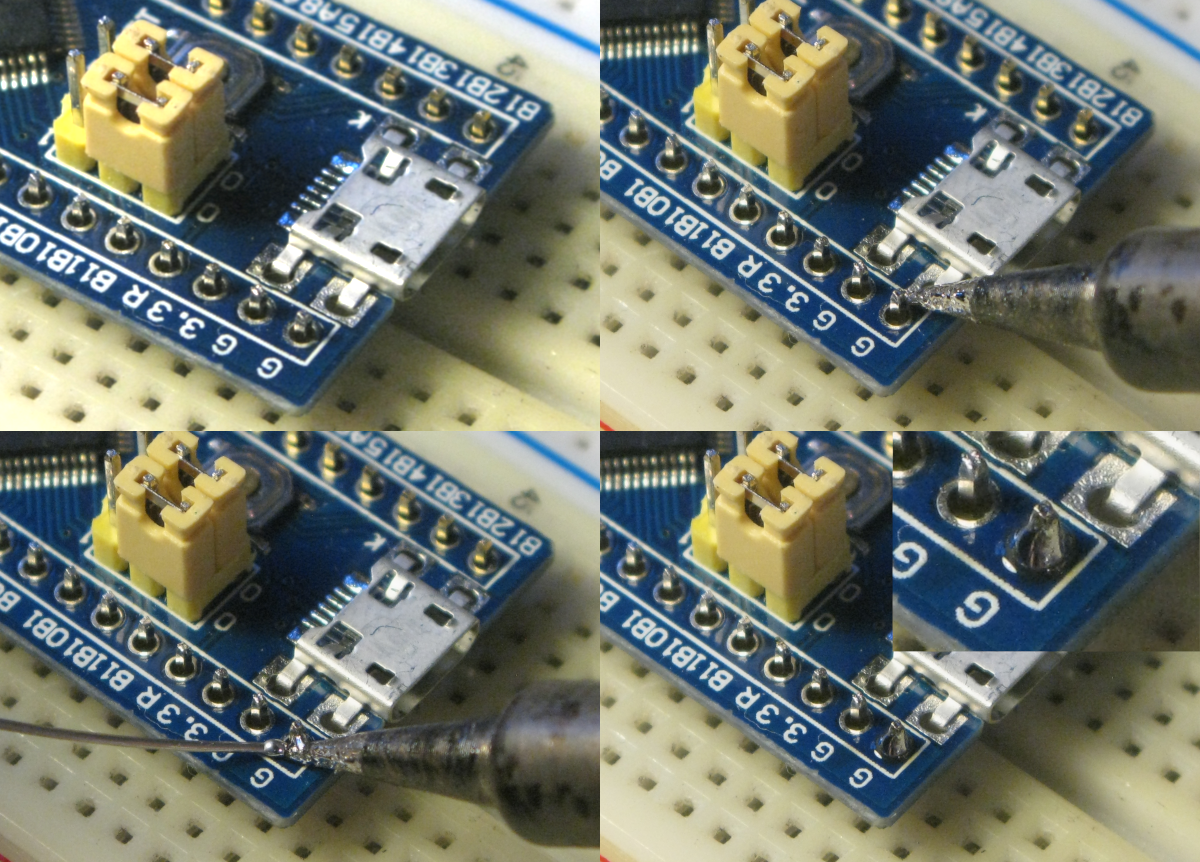
\includegraphics[width=0.99\textwidth,clip=true]{lutowanie.png}}\\
  \small
  \textbf{Lutowanie pinu mikrokontrolera.} Listwy kołkowe zostały umieszczone w płytce stykowej, aby je umiejscowić. \textit{Zaczynając od lewego górnego zdjęcia,
    zgodnie z ruchem wskazówek zegara:} Umiejscowienie pinu. Ogrzanie pinu i pola lutowniczego na płytce mikrokontrolera.
  Dotknięcie spoiwem (cyną).
  Gotowy lut (oraz jego przybliżenie).
\end{center}\end{Ramka}
\vspace*{\baselineskip}

Aby zalutować pin w otworze, najpierw dotknij grotem lutownicy
miejsca, które będziesz lutować (pola lutowniczego) oraz pinu. Trzeba ogrzać oba elementy przed ich połączeniem. Po około sekundzie, dotknij pinu końcówką odcinka cyny.
\\

Postaraj się, aby listwy kołkowe były prostopadle do płytki. Jeżeli masz odcinek damskiej listwy, możesz za jego pomocą
umiejscowić piny, które lutujesz. Możesz też użyć do tego płytki stykowej. Lutowanie zacznij od czterech pinów na rogach płytki.
\\

Kształt gotowego lutu powinien być stożkowaty. Jeżeli jest obły, oznacza to zbyt dużą ilość użytej cyny. Kuliste luty prawdopodobnie nie związały pinu z płytką (pole lutownicze nie było dobrze ogrzane). Jeśli lut nie jest błyszczący, oznacza to, że niepoprawnie związał. W takim wypadku spróbuj dodać
topnika (np. kalafonii).\\

Umiejętne lutowanie wymaga trochę praktyki, ale nie jest skomplikowane. Pamiętaj, aby lutować w dobrze wentylowanym
pomieszczeniu. Po zakończeniu umyj ręce.

\subsection{Instalacja i przygotowanie narzędzi}

Do programowania mikrokontrolera STM32 użyjemy następujących narzędzi programistycznych:

\begin{itemize}
\item Toolchain\footnotemark  dla architektury \emph{arm-none-eabi} (\Verb$gcc-arm-none-eabi$ oraz \Verb$binutils-arm-none-eabi$)
  \footnotetext{Tooolchain to zbiorowe określenie na narzędzia do przekształcania kodu źródłowego na kod maszynowy. Zawiera m.in. kompilator, linker (konsolidator), narzędzia obsługujące pliki obiektowe oraz kopujące dane między formatami plików wykonywalnych (\texttt{objcopy}) itd.}
\item Implementację libC (\Verb$libstdc++-arm-none-eabi-newlib$)
\item Narzędzie do programowania przez UART (\Verb$stm32flash$)
\item Program terminalowy do obsługi portów~szeregowych (\Verb$picocom$)
\item Bibliotekę \Verb$libopencm3$
\end{itemize}
Wszystkie narzędzia, oprócz ostatniego, dostępne są w repozytoriach Debiana (i systemów na nim opartych). Możesz je zainstalować
za pomocą polecenia:

\begin{CodeFrame*}[bash]{}
sudo apt install gcc-arm-none-eabi binutils-arm-none-eabi libstdc++-arm-none-eabi stm32flash picocom
\end{CodeFrame*}

Instalacja i kompilacja \Verb$libopencm3$ odbywa się w następujący sposób:

\begin{CodeFrame*}[bash]{}
git clone https://github.com/libopencm3/libopencm3.git
cd libopencm3
make
\end{CodeFrame*}

\subsection{Połączenie mikrokontrolera}
Aby móc uruchomić nasz kod na mikrokontrolerze, musimy podłączyć go do komputera w celu wgrywania na niego skompilowanych programów.
STM32 można programować na wiele sposobów, my będziemy używać do tego interfejsu UART\footnote{Inne z nich to SWD oraz JTAG}.\\

Aby zaprogramować mikrokontroler musisz podłączyć go do przejściówki USB-UART (nie podłączaj jeszcze
przejściówki do komputera).
Za pomocą pasujących kabelków podłącz następujące piny przejściówki do pinów na mikrokontrolerze:
\begin{itemize}
\item masę (GND) do (dowolnej) masy miktrokontrolera (GND lub G)
\item RX do TX mikrokontrolera (pin A9)
\item TX do RX mikrokontrolera (pin A10)
\item 5V do 5V mikrokontrolera
\end{itemize}

Za pomocą obcążków lub pęsety przełóż górną (patrząc na mikrokontroler tak aby port USB był po lewej) zworkę na
pozycję ``1''.

Sprawdź wszystkie połączenia i podłącz przejściówkę do portu USB komputera. Na mikrokontrolerze powinna zaświecić się tylko czerwona dioda
\texttt{PWR}

Możesz sprawdzić połączenie z mikrokontrolerem używając \Verb$stm32flash$ do obliczenia sumy kontrolnej pamięci mikrokontrolera.
Jeżeli polecenie poniżej nie zgłosi błędów, oznacza to, że wszystko działa poprawnie.

\begin{CodeFrame*}[bash]{}
stm32flash -C /dev/ttyUSB0
\end{CodeFrame*}

Tak przygotowany mikrokontroler jest gotowy do pracy.


\section{Płytka stykowa}
Płytka stykowa pozwala na szybkie prototypowanie układów bez konieczności lutowania. Składa się ona z macierzy dziurek,
pod którymi są umieszczone blaszki łączące sąsiednie dziurki. Blaszki są umieszczone w taki sposób, aby łączyły wszystkie
5 dziurek w kolumnie. Dzięki temu zamiast budować prototypy lutując je na uniwersalnych płytkacj drukowanych, wystarczy, że
umieścimy nasze elementy w otworkach płytki stykowej. 
\\

Przez środek płytki przechodzi wyżłobienie bez dziurek. Otworki w tej samej kolumnie, ale po przeciwnych jego
stronach nie są ze sobą połączone elektrycznie. Służy ono do umieszczania tam układów scalonych w obudowach DIP.
Układy wkłada się ``okrakiem'' nad tym odstępem, tak aby każda z nóżek trafiła do dziurki w oddzielnej kolumnie.
Typowo, po wyprodukowaniu w fabryce, nóżki układów scalonych są rozgięte do zewnątrz. Jeżeli układ nie pasuje do płytki,
to trzeba je troche dogiąć.
Najłatwiej jest doginać jedną stronę na raz, na przykład o blat stołu. Nie należy doginać nóżek pojedynczo, np. za pomocą obcążków.
Nie powinno się też nadmiernie ich rozginać, ponieważ po kilkunastu zgięciach mogą odpaść.
\\

\begin{Ramka}{}\begin{center}
  \noindent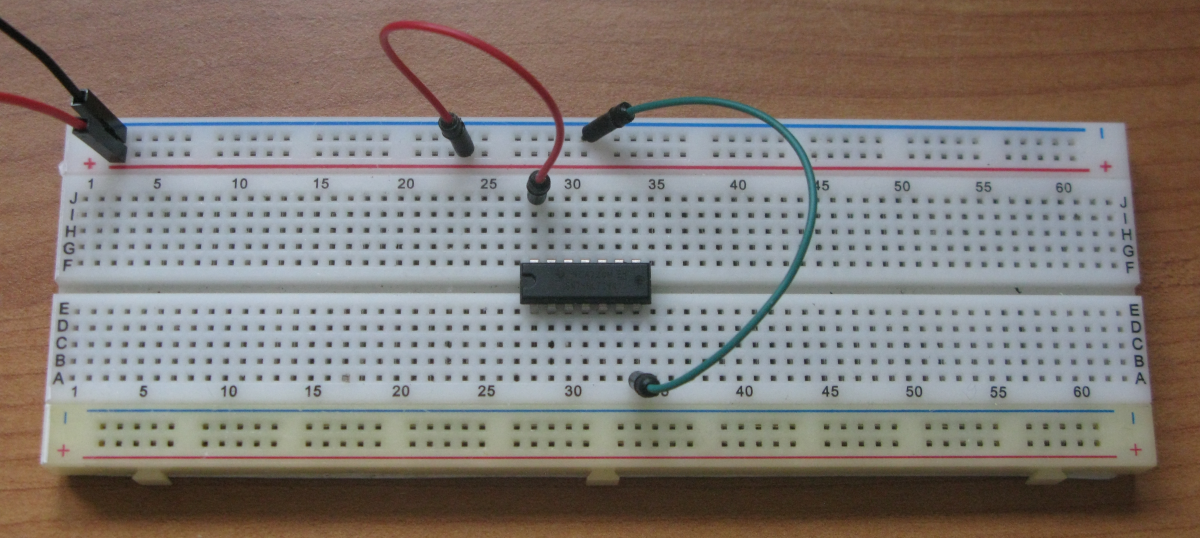
\includegraphics[width=0.95\textwidth]{dip_ic.png}\\
  Tak umieszczamy układy scalone w płytce stykowej. Dzięki temu każdy z pinów ma połączenie z oddzielną kolumną otworków na płytce.
\end{center}\end{Ramka}

Umieszczając inne elementy w płytce stykowej należy pamiętać, jak połączone są otworki - to znaczy, że jeżeli chcemy
połączyć dwa elementy, to ich odpowiednie ``nóżki'' muszą być umieszczone w tej samej kolumnie. Można też połączyć dwie kolumy otworków
ze sobą za pomocą pasujących kabelków.
\\

Na brzegach płytki najczęściej znajdują się podłużne listwy z takimi samymi otworkami, co reszta płytki, pogrupowanymi w grupy 2x5.
Niektóre płytki posiadają też nadrukowane kreski oraz znaki + i -. Te listwy służą do doprowadzania
zasilania do układu na płytce. Otworki w jednej linii wzdłuż płytki są połączone elektrycznie - tworzą tzw.
\textbf{szynę zasilania}. Z reguły umieszczane są w parach - jedna szyna dla dodatniego napięcia, a druga dla ujemnego (masy).\\

Jeżeli twoja płytka ma nadrukowane oznaczenia wzdłuż tych szyn, to napięcia zasilania (+ oraz -) z przetwornicy należy podłączać zgodnie z~tymi
oznaczeniami. Zmniejsza to ryzyko kosztownej pomyłki.\\

W niektórych płytkach szyny zasilania są rozdzielone w połowie. Należy o tym pamiętać, ponieważ nie ma na to reguły.
Możesz sprawdzić czy Twoja płytka ma rozdzielone szyny za pomocą multimetru (w trybie omomierza lub testu przewodnictwa). Pozwoli to uniknąć
niespodzianek przy prototypowaniu.

\begin{ProTip}{\normalfont{\strong{Uwaga}}}
  Przed wprowadzaniem jakichkolwiek zmian na płytce stykowej odłącz zasilanie. Pozwoli to uniknąć przypadkowych zwarć i uszkodzeń elementów.
\end{ProTip}

\begin{Zadanie}{}{}
  Za pomocą funkcji testu połączeń swojego miernika, sprawdź, czy Twoja płytka stykowa ma rozdzielone szyny zasilania.
  \textit{Wskazówka: Użyj odpowiednich kabelków żeby podłączyć sondy miernika do szyn na płytce - jeden koniec kabelka włóż do płytki a drugim
    dotknij do sondy miernika.}
\end{Zadanie}

\begin{Zadanie}{}{}
  Znajdź w swoim zestawie opornik 1k$\Omega$ (możesz użyć do tego multimetru, ale pamiętaj, że oporniki mają typową tolerancję 5\Verb$%$,
  więc jest mało prawodopodobne, że znajdziesz opornik który ma dokładnie 1000$\Omega$). Jaki prąd popłynie, gdy podłączysz go do napięcia 9V?
  Potwierdź swoje obliczenia za pomocą pomiaru multimetrem.
\end{Zadanie}

\begin{Zadanie}{}{}
  Jaka moc wydzieli się na oporniku z poprzedniego zadania?
\end{Zadanie}


\section{Układy scalone}
\textbf{Układy scalone} pozwalają szybko i sprawnie konstruować skomplikowane układy elektroniczne przy minimum nakładu i kosztu. Dzięki nim możemy
używać gotowych bloków cyfrowych (np. licznik, sumator, bramka logiczna) oraz analogowych (regulator napięcia, wzmacniacz operacyjny,
przełączniki anlogowe itp.) zamiast budować je od postaw z \textbf{elementów dyskretnych} (transyzstory, oporniki itp.). Produkowane są
układy o bardzo różnych stopniach integracji - od bardzo niskich, takich jak np. bramki logiczne, do bardzo wysokich, jak np. gotowe komputery
(tzw. SoC - system on a chip).
\\

Układ scalony posiada od kilku do kilkudziesięciu wyprowadzeń które służą do łączenia go z innymi elementami układu elektronicznego.
Każde z tych wyprowadzeń pełni określoną funkcję (zasilanie, wejścia, wyjścia itp.). W karcie~katalogowej danego układu scalonego wszystkie
piny są ponumerowane, nazwane a ich funkcje opisane.
\\

Na razie skupimy się na prostszych układach, które możesz umieścić w swojej płytce stykowej - układach, które produkowane są w obudowach DIP.
Charakteryzuje się ona prostopadłymi, szeroko (w porównaniu do innych obudów) rozstawionymi pinami które można łatwo umieścić w płytce stykowej.

\begin{wrapfigure}{r}{0.25\textwidth}
  \begin{center}
    \vspace{-20pt}
    \includegraphics[height=0.25\textwidth,angle=90,origin=c]{img/elektronika/DIP14}
    \vspace{-40pt}
    
    \small{14-pinowa obudowa DIP, widok z~góry}
    \vspace{-33pt}
  \end{center}
\end{wrapfigure}

W obudowie typu DIP, oznaczenie pinu 1. ma formę wklęsłego wcięcia na jednym z końców układu, lub kropki na narożniku. W przypadku tego drugiego, pin przy którym znajduje się kropka to pin nr 1. W przypadku wcięcia, pin nr 1 to lewy dolny, patrząc na układ obrócony oznaczonym końcem w lewo, napisami na obudowie w Twoją stronę. Kolejne piny liczy się idąc przeciwnie do ruchu wskazówek zegara. Przedstawia to rysunek obok.
Przy podłączaniu układu scalonego ważne jest aby nie pomylić numerów pinów (nóżek). Każdy z nich ma z góry określoną funkcję.

\begin{ProTip}{\normalfont{\strong{Wskazówka}}}
  W elektronice do wyrażania wymiarów stosuje się m.in. jednostkę \textbf{mil}\footnote{zwaną też \textit{thou}, od \textit{thousands of an inch}},
  równą 1/1000 cala. Rozstaw nóżek w obudowie DIP to 100 mili (= 2.54 mm). Taki sam jest również rozstaw otworków na płytce stykowej.
\end{ProTip}


\section{Zadania dodatkowe}

\vspace{13pt}
\begin{center}\includegraphics[width=0.6\textwidth]{img/elektronika/praca_domowa-szeregowe_rownolegle}\end{center}
\vspace{-7pt}

\begin{Zadanie}{}{}
  Rezystory $R_1$ i $R_2$ połączone zostały szeregowo i podłączone do źródła napięcia U, tak jak pokazano na powyższym schemacie.
  \begin{enumerate}[label=\alph*)]
    \item Zapisz zależność (wzór) określający spadek napięcia na rezystorze $R_1$.
    \item Zapisz zależność (wzór) określający sumaryczną moc, która wydzieli się na obu tych rezystorach.
  \end{enumerate}
\end{Zadanie}

\begin{Zadanie}{}{}
  Rezystory $R_3$ i $R_4$ połączone zostały równolegle i podłączone do źródła napięcia U, tak jak pokazano na powyższym schemacie.
  \begin{enumerate}[label=\alph*)]
    \item Zapisz zależność (wzór) określający prąd płynący przez rezystor $R_3$.
    \item Zapisz zależność (wzór) określający łączną rezystancję obu rezystorów (czyli ich rezystancję zastępczą).
  \end{enumerate}
\end{Zadanie}

\begin{Zadanie}{}{}
  Znajdź dokumentację (kartę katalogową) do rejestru przesuwnego, który kupiłeś/aś (CD4094 lub 74HC595).
  Odczytaj, jakie jest największe napięcie zasilania tego układu (\textit{supply voltage}, w sekcji
  \textit{Absolute maximum ratings}), oraz do których pinów należy podłączać napięcie zasilania (w sekcji \textit{pin configuration}).
\end{Zadanie}


\copyrightFooter{
	© Matematyka dla Ciekawych Świata, 2020.\\
	© Robert Ryszard Paciorek <rrp@opcode.eu.org>, 2020.\\
	© Krzysztof Lasocki <krz.lasocki@gmail.com>, 2020.\\
	Kopiowanie, modyfikowanie i redystrybucja dozwolone pod warunkiem zachowania informacji o autorach.
}

\end{document}
